\chapter{Příklad definice typu komponenty}
\label{lst:createtype}

Výpis demonstruje registraci typu komponenty \texttt{heading}. Typ je registrován rozšířením základního typu komponenty pomocí parametru \texttt{extend}, čímž automaticky přebírá sdílenou logiku -- konkrétně synchronizaci atributu \texttt{data-oidis-bind}, správu parametru odpovídajícího za volbu importované třídy ve výsledném souboru a obsluhu příslušných událostí. Parametr \texttt{extendFn} zajišťuje, že inicializační metoda základního typu je při vytvoření instance volána, a nikoli nahrazena vlastní implementací. Funkce \texttt{isComponent} určuje pravidlo rozpoznání: pokud editor při parsování HTML narazí na prvek H1 až H6, automaticky jej přiřadí k tomuto typu. Tím je zajištěno správné načtení komponenty při importu existujícího souboru.

V sekci \texttt{model} jsou definovány výchozí hodnoty komponenty, jako jsou tag, obsah a~interní vlastnosti typu. Pole \texttt{traits} odpovídá za vlastnosti nabízené uživateli v panelu nastavení vizuálního editoru -- v tomto konkrétním případě přidává výběr úrovně nadpisu ze~seznamu. Pole \texttt{allTraits} obsahuje obecné vlastnosti sdílené všemi typy komponent, jako jsou Bootstrap utility třídy pro flexbox, odsazení nebo viditelnost. Metoda \texttt{init} synchronizuje hodnotu interní vlastnosti s aktuálním tagem při načtení komponenty do editoru, metoda \texttt{updated} reaguje na změnu hodnoty v panelu vlastností a aktualizuje stav prvku~--~například změní jeho tag bez nutnosti přímého zásahu do HTML kódu.

\begin{lstlisting}[
  float=h,
]
editorTypes.addType("heading", {
        extend: "base-component",
        extendFn: ["init"],
        isComponent: (el) =>
            /^H[1-6]$/.test(el.tagName) ? { type: "heading" } : false,

        model: {
            defaults: {
                tagName: "h1",
                content: "Heading",
                headingLevel: "h1",
                importGeneration: [GuiCommonsImport],
                traits: [
                    {
                        type: "select",
                        name: "headingLevel",
                        label: "Level",
                        category: GeneralCategory,
                        changeProp: 1,
                        options: [
                            { id: "h1", label: "H1", value: "h1" },
                            { id: "h2", label: "H2", value: "h2" },
                            { id: "h3", label: "H3", value: "h3" },
                            { id: "h4", label: "H4", value: "h4" },
                            { id: "h5", label: "H5", value: "h5" },
                            { id: "h6", label: "H6", value: "h6" }
                        ]
                    },
                    ...allTraits
                ]
            },

            init() {
                this.set("headingLevel", this.get("tagName"));
            },

            updated(property, value) {
                if (property === "headingLevel" && value) {
                    this.set("tagName", value);
                }
            }
        }
    });
\end{lstlisting}

\chapter{Příklad třídy komponenty projektu postaveného na frameworku Oidis}
\label{lst:file}

Výpis ukazuje strukturu souboru komponenty, se kterou Oidis Studio pracuje. Třída komponenty dědí ze základní třídy \texttt{BasePanel} a obsahuje importy použitých tříd, deklarace a~inicializaci proměnných odpovídajících interaktivním prvkům uživatelského rozhraní a~metodu \texttt{innerHtml} vracející HTML šablonu komponenty.

V souboru jsou vyznačeny dvojice komentářů, které ohraničují bloky spravované editorem. Tyto komentáře slouží jako značky, podle nichž editor při načtení souboru rozpozná, odkud má převzít HTML obsah pro zobrazení na editační ploše, a podle nichž při uložení vloží nově vygenerovaný kód. Blok importů vymezuje místo, kam jsou doplňovány importy tříd použitých pro proměnné propojené s aplikační logikou. Bloky deklarací a inicializace ohraničují části kódu odpovídající za vytvoření těchto proměnných. Poslední blok pak vymezuje samotnou HTML šablonu komponenty, ve které jsou prvky propojeny s deklarovanými proměnnými prostřednictvím atributu \texttt{data-oidis-bind}.

Kód mimo vyznačené bloky zůstává bez změn a editor do něj nezasahuje. Sem patří zejména obchodní logika, vlastní metody třídy nebo doplňkové proměnné, které nesouvisí s vizuálním návrhem komponenty.

Aplikace má možnost zpracovat i soubor neobsahující vyhrazené značky. Na základě klíčových slov a předpokládaného umístění jednotlivých bloků načte HTML obsah do editoru a identifikuje odpovídající proměnné použité v této struktuře. Při exportu následně doplní vymezení bloků a zapíše do nich generovaný obsah, přičemž proměnné nesouvisející s propojením na HTML prvky i ostatní kód vytvořený vývojářem zůstávají beze změny.
\begin{lstlisting}[
  float=h,
  breaklines=true,
  breakatwhitespace=true
]
import { BasePanel } from "./../../../../Io/Oidis/Gui/Bootstrap/Primitives/BasePanel.js";
//generated imports start
import {Button} from
"@io-oidis-usercontrols/.../UserControls/Bootstrap/UserControls/Button.js";
//generated imports end
...other imports
            
export class NewComponent extends BasePanel {
    //generated variables start
    public readonly importButton : Button;
    public readonly saveButton : Button;
    //generated variables end
    private count : number;
            
    constructor() {
    super();
    //generated inicialization start
    this.importButton = new Button();
    this.saveButton = new Button();
    //generated inicialization end
    this.count = 0;
    }

    public setCount(newCount : number) : void {
        this.count = newCount;
    }
            
    protected innerHtml() : string {
       //generated html start
       return `    
  <div class="d-flex justify-content-between align-items-center p-2">
    <div>
      <img alt="Logo" src="/resource/graphics/.../MainPage/Logo.svg" class="img-fluid"/>
      <span>Oidis Studio</span>
    </div>
    <div>
      <button type="button" data-oidis-bind="${this.importButton}" class="btn btn-primary">Importovat html</button>
      <button type="button" data-oidis-bind="${this.saveButton}" class="btn btn-primary">Uchovat zmeny</button>
    </div>
  </div>
        `;
        //generated html end
    }
}
\end{lstlisting}


\chapter{Snímky obrazovky}
\label{screen}
\begin{figure*}[h]\centering
  \centering
  \includegraphics[width=\linewidth]{obrazky-figures/screen.png}\hfill
  \caption{Snímek obrazovky Oidis Studio. Levá část obsahuje katalog komponent a~strom HTML prvků. Centrální část tvoří editační plocha s náhledem komponenty včetně ovládacích nástrojů a editor kódu s aktuálním stavem výsledné HTML struktury. Pravá část obsahuje panel vlastností vybraného prvku a jeho stylování.}
\end{figure*}

\begin{figure*}[h]\centering
  \centering
  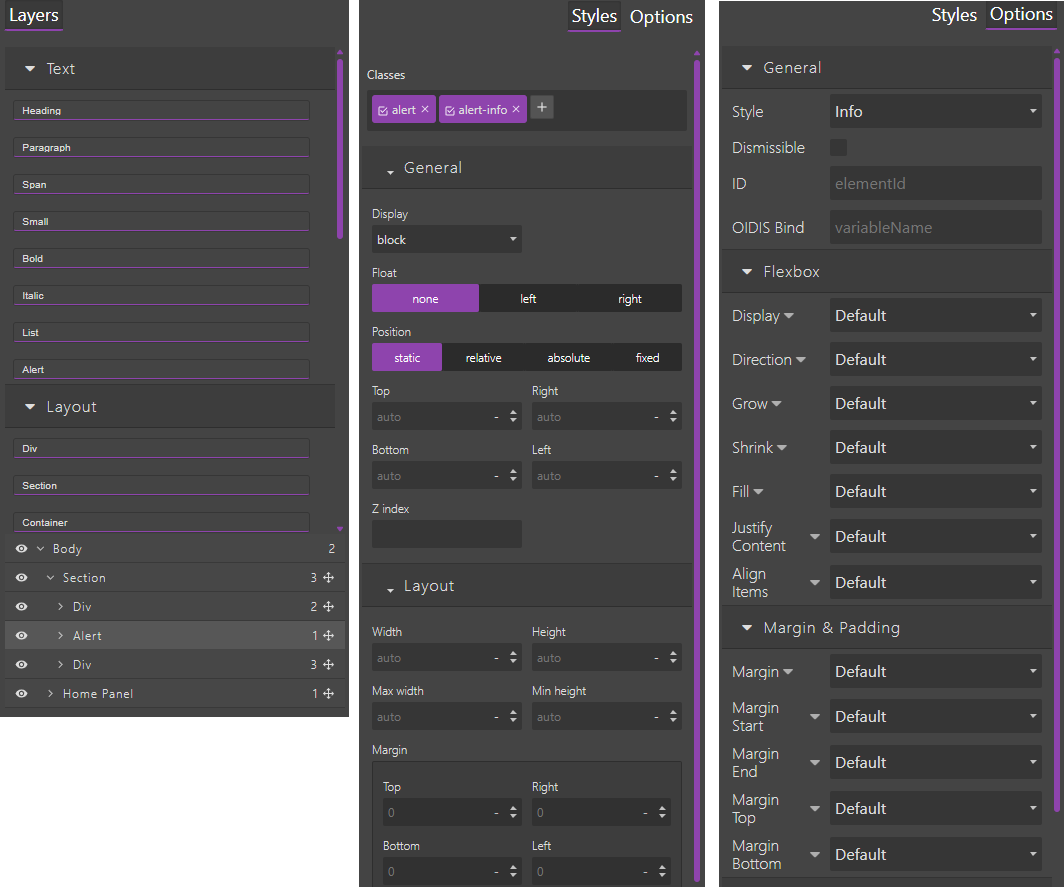
\includegraphics[width=\linewidth]{obrazky-figures/Panels.png}\hfill
  \caption{Snímky jednotlivých ovládacích panelů. Levý panel obsahuje katalog komponent a stromovou reprezentaci HTML prvků. Centrální panel zobrazuje nastavení stylů vycházející ze standardní konfigurace knihovny GrapesJS. Pravý panel slouží k nastavení vlastností vybraného prvku. Kategorie \texttt{General} obsahuje specifická nastavení komponenty, zatímco další kategorie obsahují obecná nastavení společná pro všechny prvky.}
\end{figure*}

\begin{figure*}[h]\centering
  \centering
  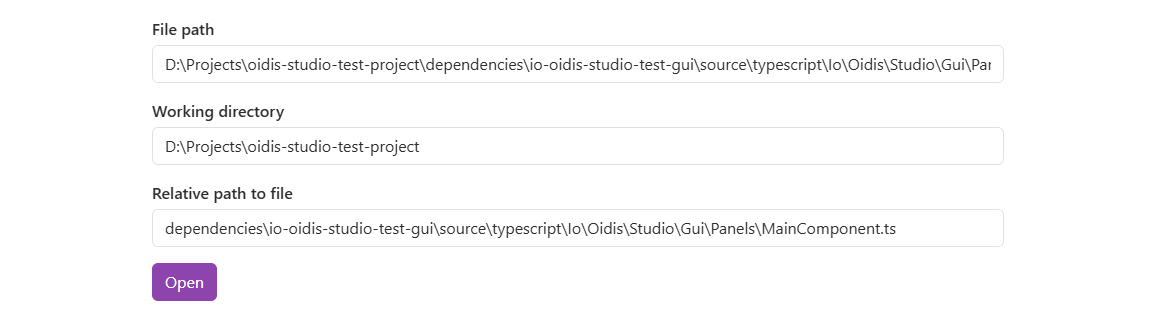
\includegraphics[width=\linewidth]{obrazky-figures/Dialog.png}\hfill
  \caption{Snímek dialogu pro zadávání cesty k požadovanému souboru.}
\end{figure*}